\documentclass[10pt,xcolor=pdflatex,hyperref={unicode}]{beamer}
\usepackage{newcent}
\usepackage[utf8]{inputenc}
\usepackage[czech]{babel}
\usepackage[T1]{fontenc}
\usepackage{hyperref}
\usepackage{fancyvrb}
\usetheme{FIT}
\usepackage{listings}
\usepackage{appendixnumberbeamer}
\lstdefinelanguage{Gherkin}{
	morekeywords = {
		Given,
		When,
		Then,
		And,
		Scenario,
		Feature,
		But,
		Background,
		Scenario Outline,
		Examples,
		Start,
		Action,
		State,
		OCR,
	},
	basicstyle=\ttfamily,
	sensitive=true,
	morecomment=[l]{\#},
	morestring=[b]",
	morestring=[b]',
	breaklines=true,
	showspaces=false,
    showstringspaces=false
}

%%%%%%%%%%%%%%%%%%%%%%%%%%%%%%%%%%%%%%%%%%%%%%%%%%%%%%%%%%%%%%%%%%
\title[Martin Krajňák - DIP]{Automatické generování testů pro GNOME GUI aplikace z metadat AT-SPI}

\author[]{Bc. Martin Krajňák}

\institute[]{
xkrajn02@fit.vutbr.cz
\\
Vedúci práce: prof. Ing. Tomáš Vojnar, Ph.D. 
\\
Odborný vedúci: Ing. Tomáš Pelka 
\\
Zadávateľ: Red Hat Czech s.r.o.

}
%\institute[]{Fakulta informačních technologií
%Vysokého učení technického v Brně\\
%Bo\v{z}et\v{e}chova 1/2. 612 66 Brno - Kr\'alovo Pole\\
%login@fit.vutbr.cz}

% České logo - Czech logo
% beamerouterthemeFIT.sty řádek 9: fitlogo1_cz

% \date{January 26, 2020}
\date{\today}
%\date{} % bez data / without date

%%%%%%%%%%%%%%%%%%%%%%%%%%%%%%%%%%%%%%%%%%%%%%%%%%%%%%%%%%%%%%%%%%

\setbeamersize{text margin left=0.5cm,text margin right=0.5cm}
\begin{document}

\frame[plain]{\titlepage}

\begin{frame}\frametitle{Cieľ práce}
    \begin{block}{\textbf{Nástroj na automatické generovanie automatizovaných testov}}

    \begin{itemize}
    \item Systematické generovanie testov na základe dostupných vykonateľných akcií GUI aplikácie cez technológiu AT-SPI
    \vspace{3mm}
    \item Využitie vstavenej podpory asistenčných technológii pre GTK/GNOME aplikácie -- AT-SPI
    \begin{itemize}
        \item \emph{strom prvkov, obsahuje metadáta a vykonateľné akcie}
    \end{itemize}
    \vspace{3mm}
    \item Využitie technológie \textit{OCR (Tesseract)}
    \begin{itemize}
        \item \emph{verifikácia extrahovaného znakov/textu z obrázkov}
    \end{itemize}
    \vspace{2mm}
    \item Zjednodušenie/zrýchlenie procesu vývoja a údržby automatizovaných testov
    \vspace{2mm}
    \item Rýchle zistenie závažných chýb v nových verziách aplikácií
    \end{itemize}

    \end{block}
\end{frame}

\begin{frame}[fragile]\frametitle{Navrhované riešenie}

\begin{itemize}
\item Black-box testovanie GUI aplikácie na základe postupne vytvoreného modelu aplikácie z metadát AT-SPI
\end{itemize}

 \begin{figure}[h]
        \center{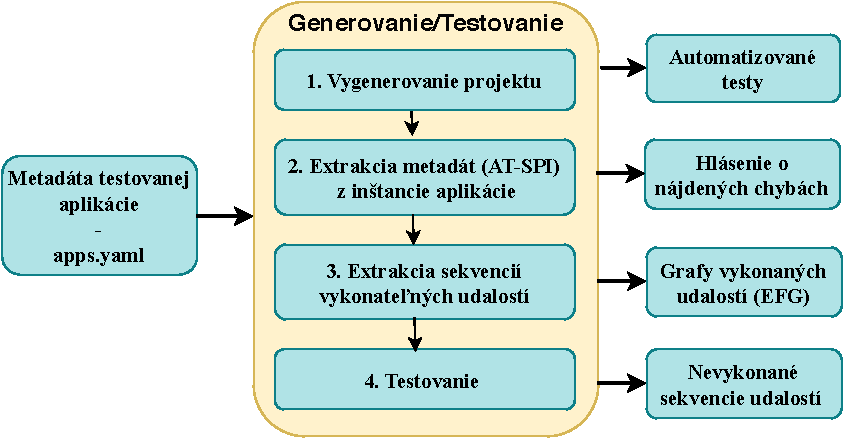
\includegraphics[width=1\textwidth]{img/diag.pdf}}
 \end{figure}
\end{frame}



\begin{frame}[fragile]\frametitle{Implementácia navrhovaného nástroja}

\begin{itemize}

\item Identifikácia prvkov aplikácie určených k interakcii s používateľom

\vspace{3mm}
\item Odvodenie sekvencií udalostí, ktoré budú postupne použité na testovanie aplikácie

\vspace{3mm}
\item Sledovanie stavu aplikácie a detekcia chýb

\vspace{3mm}
\item Export testov
\vspace{3mm}
\item Rozšírenie testovacej knižnice \textit{qecore} používanej na testovanie aplikácii v prostredí GNOME
\begin{itemize}
    \item \emph{podpora pre aplikácie typu Flatpak}
    \item \emph{pridanie nových parametrov}
    \item \emph{navrhnuté zmeny boli schválené a sú súčasťou testovacej knižnice}
\end{itemize}
\end{itemize}
\end{frame}



\begin{frame}[fragile]\frametitle{Integrácia a optimalizácia technológie OCR}
\begin{itemize}
\item Dodatočná verifikácia reťazcov extrahovaných z AT-SPI stromu
\item Prevod obrázka do formy, v ktorej sú optimálne podmienky pre rozpoznávanie textu cez \textit{OCR (Tesseract)} -- čierny text na bielom pozadí
\item Škálovanie/zvýšenie rozlišenia obrázka
\end{itemize}
 \begin{figure}[h]
        \center{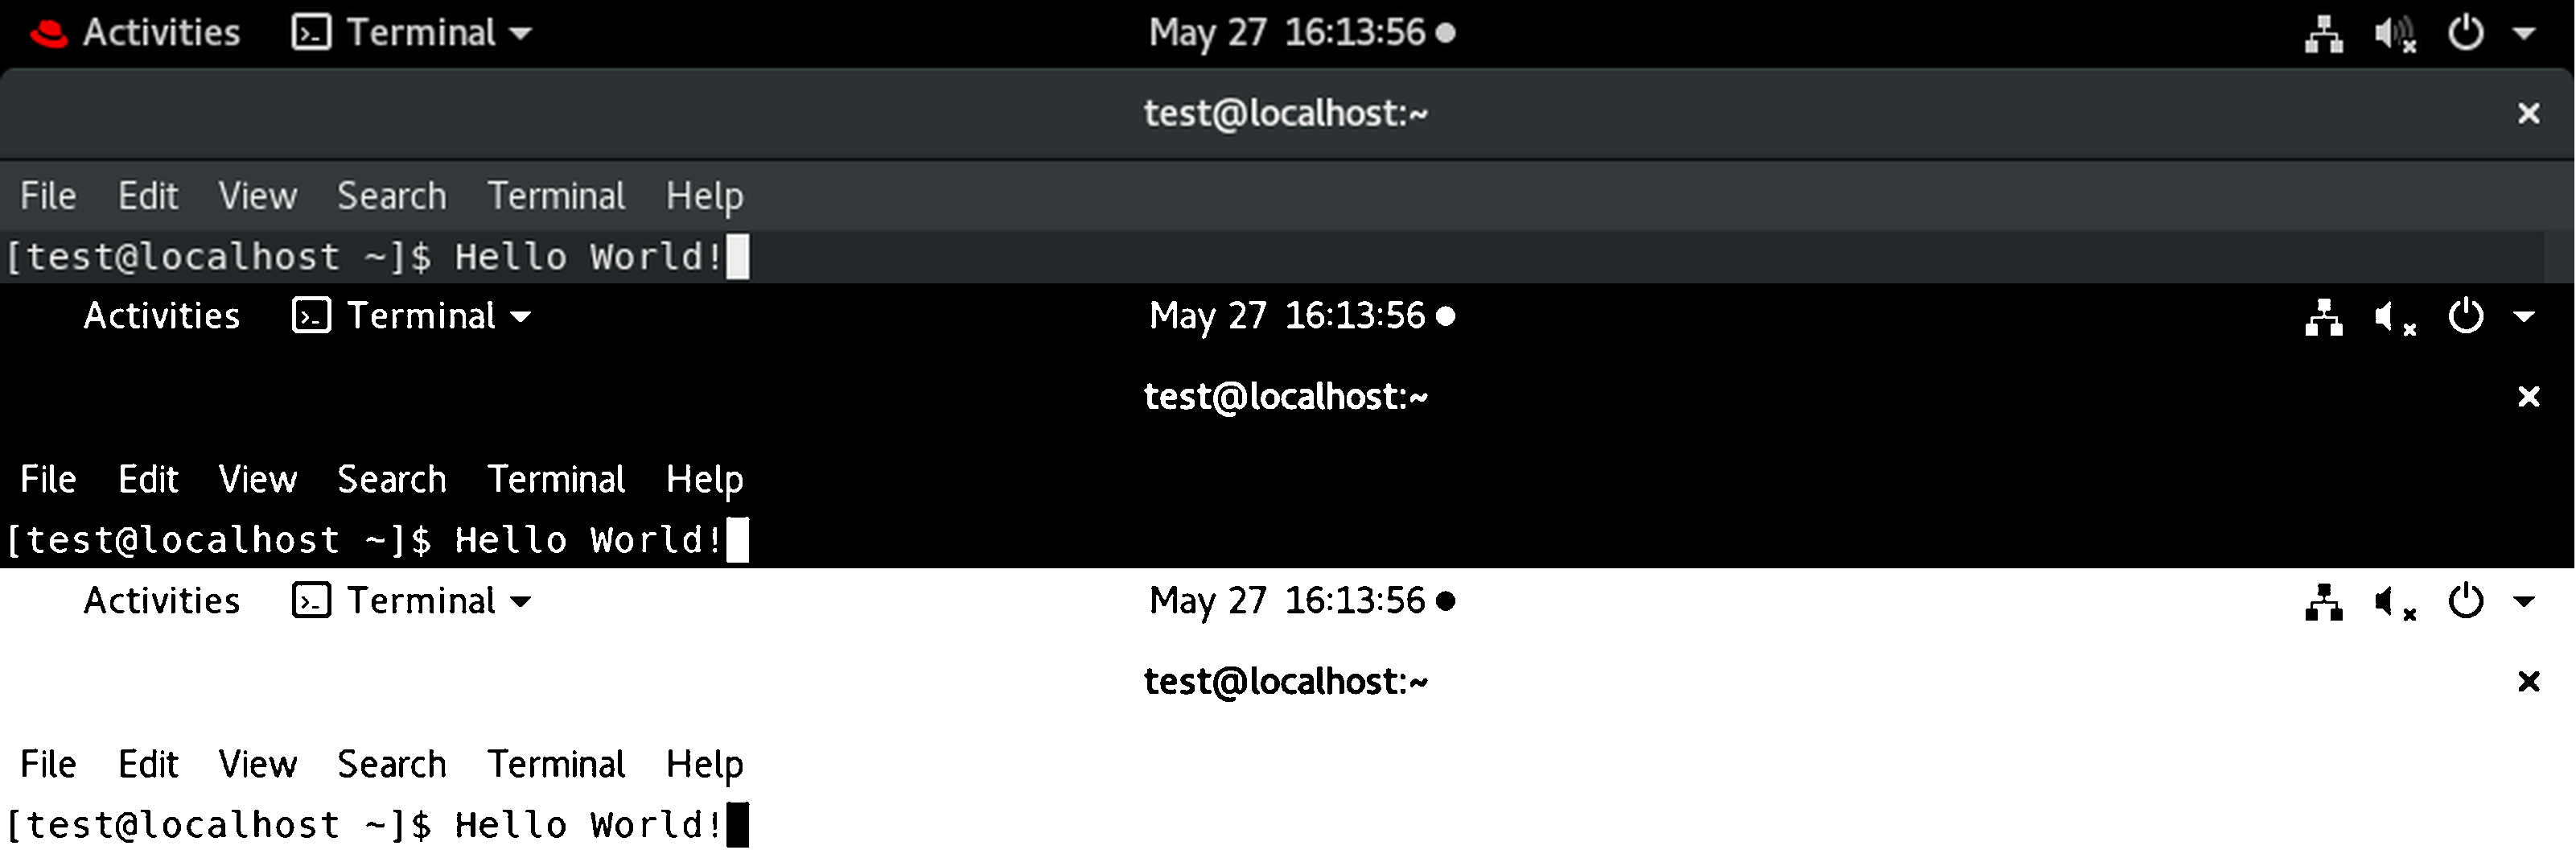
\includegraphics[width=1\textwidth]{img/OCR_conversion.png}}
 \end{figure}

\end{frame}


\begin{frame}[fragile]\frametitle{Práca generátora s aplikáciou: EFG I}
\begin{itemize}
    \item EFG vygenerovený po prvotnom naskenovaní aplikácie \textit{GNOME~Help}
    \item Graf zobrazuje 96 vykonateľných udalostí 78 uzloch (grafických prvkoch aplikácie).
\end{itemize}
\begin{figure}[h]
        \center{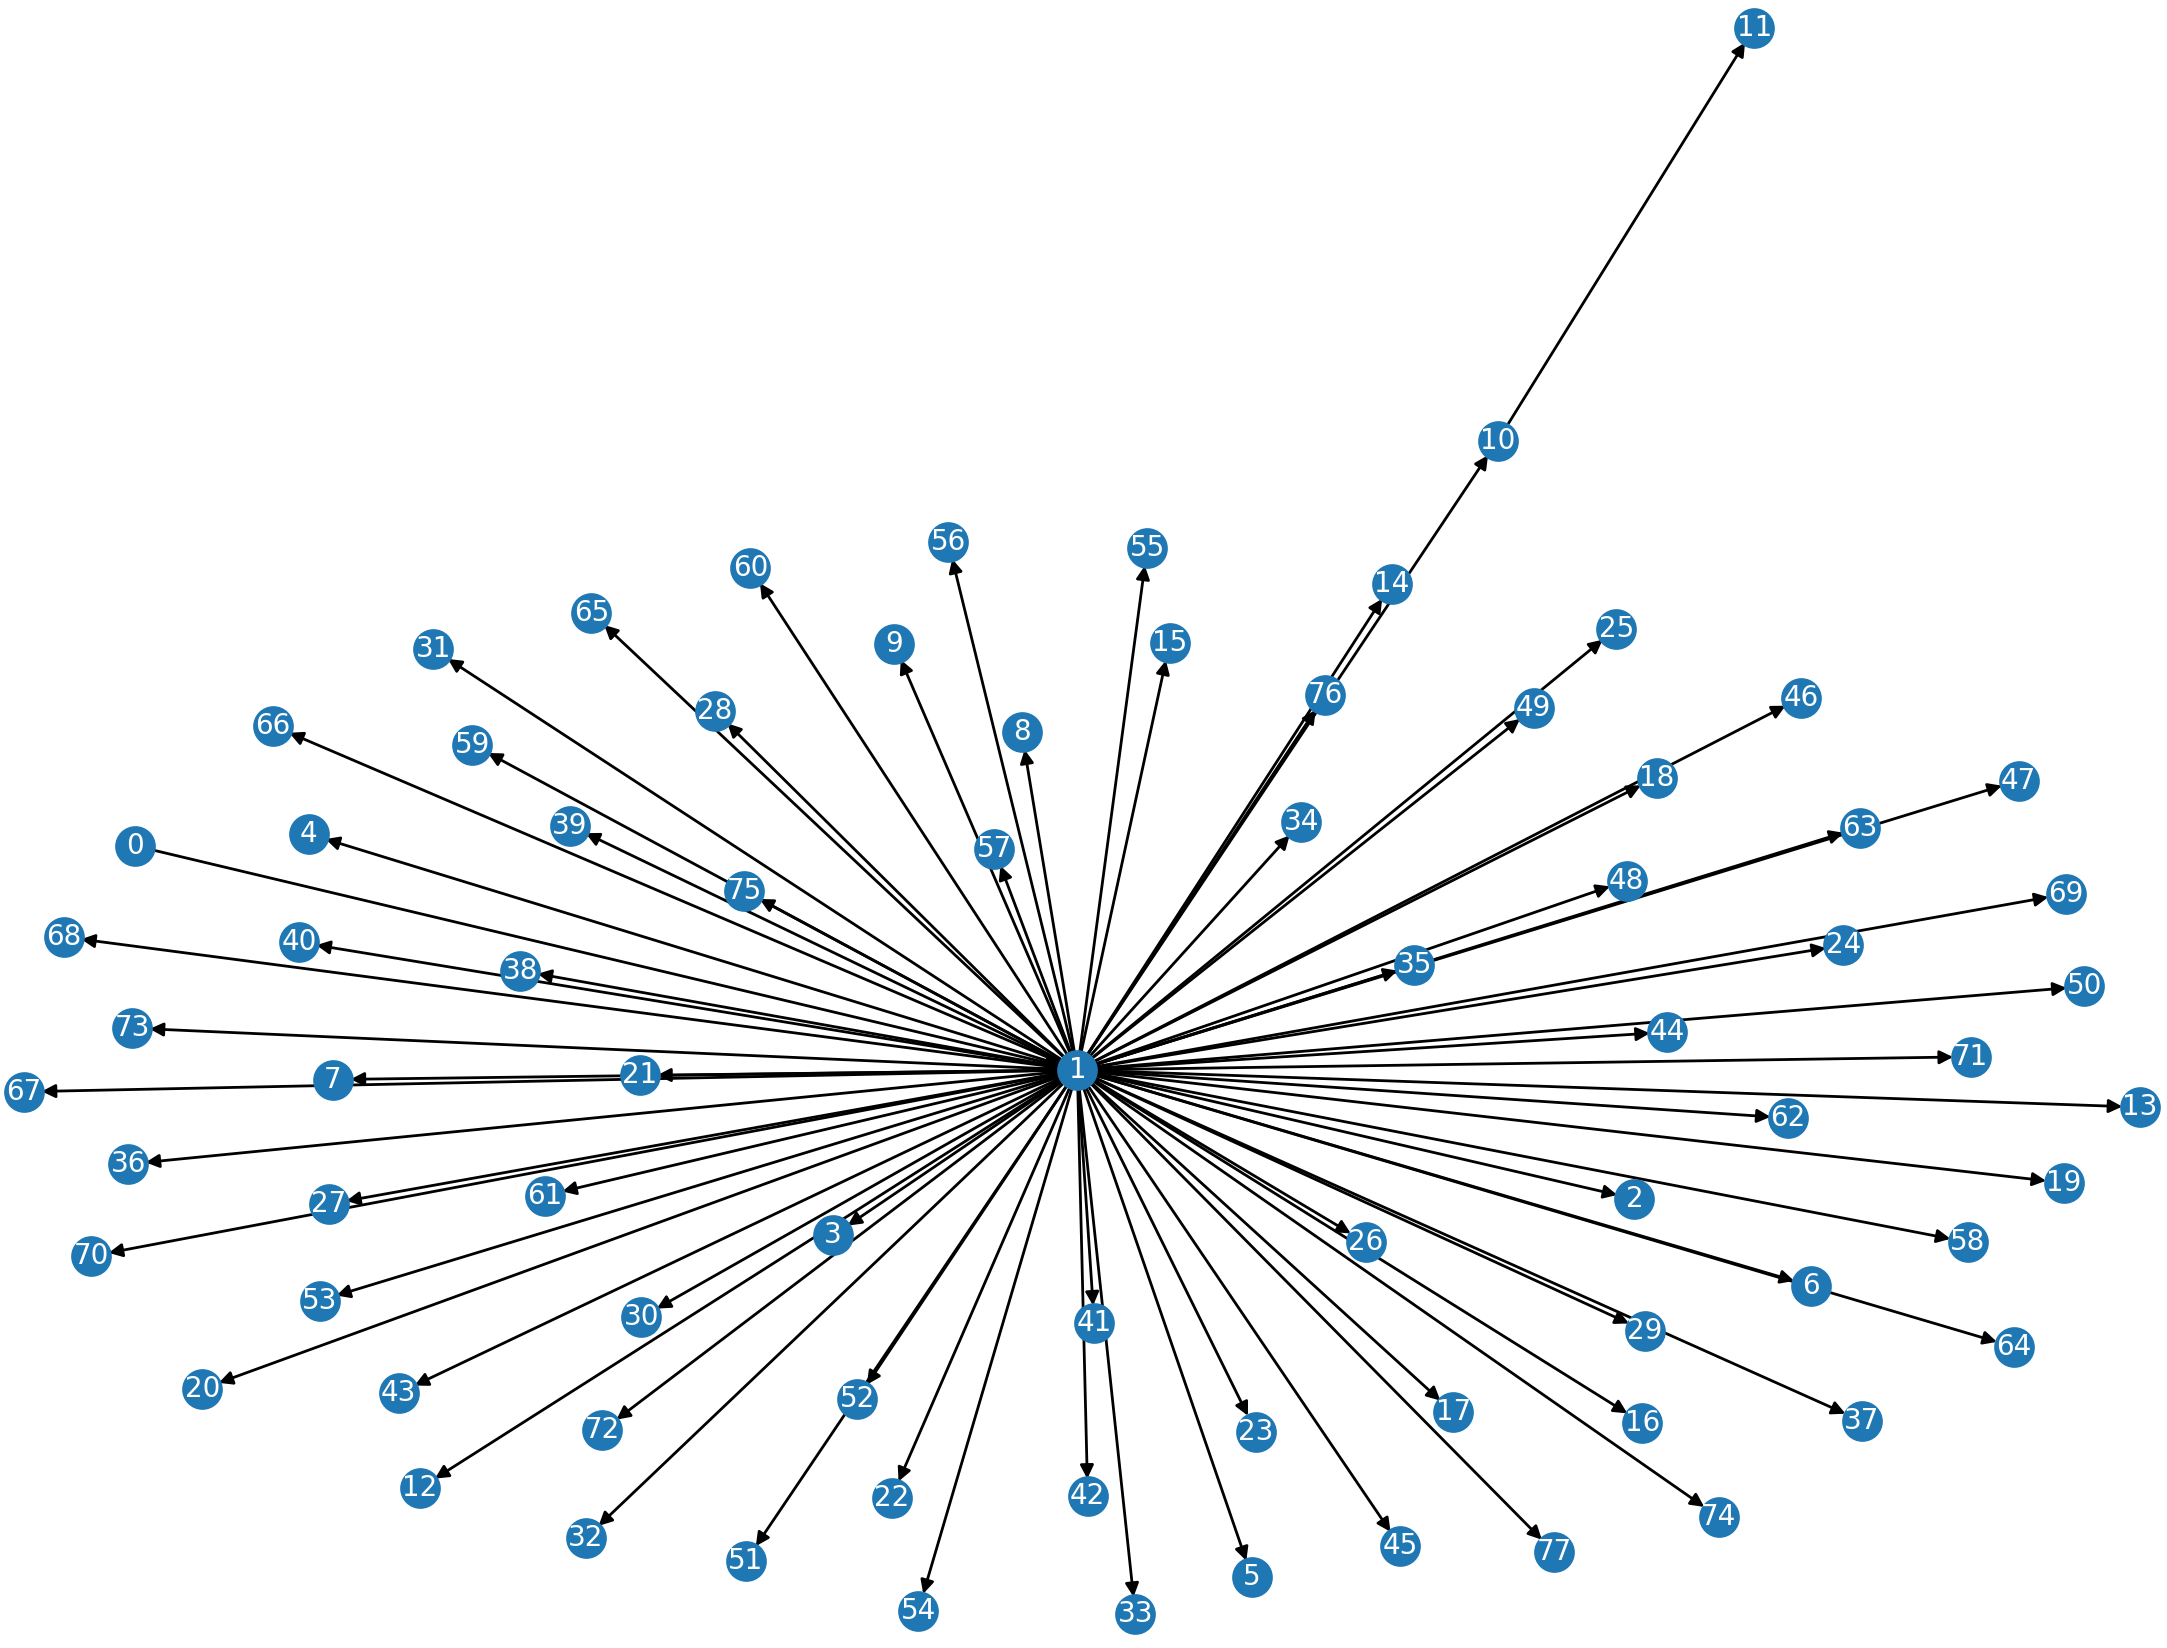
\includegraphics[width=0.7\textwidth]{img/yelp_n_start.png}}
 \end{figure}

\end{frame}

\begin{frame}[fragile]\frametitle{Práca generátora s aplikáciou: EFG II}

\begin{itemize}
    \item EFG vygenerovený po dokončení testovania \textit{GNOME~Help}
    \item Graf zobrazuje 4696 udalostí vykonaných na 2415 uzloch
    \item Demoštrácia práce generátora s novonájdenými sekvenciami udalostí 
\end{itemize}

\begin{figure}[h]
        \center{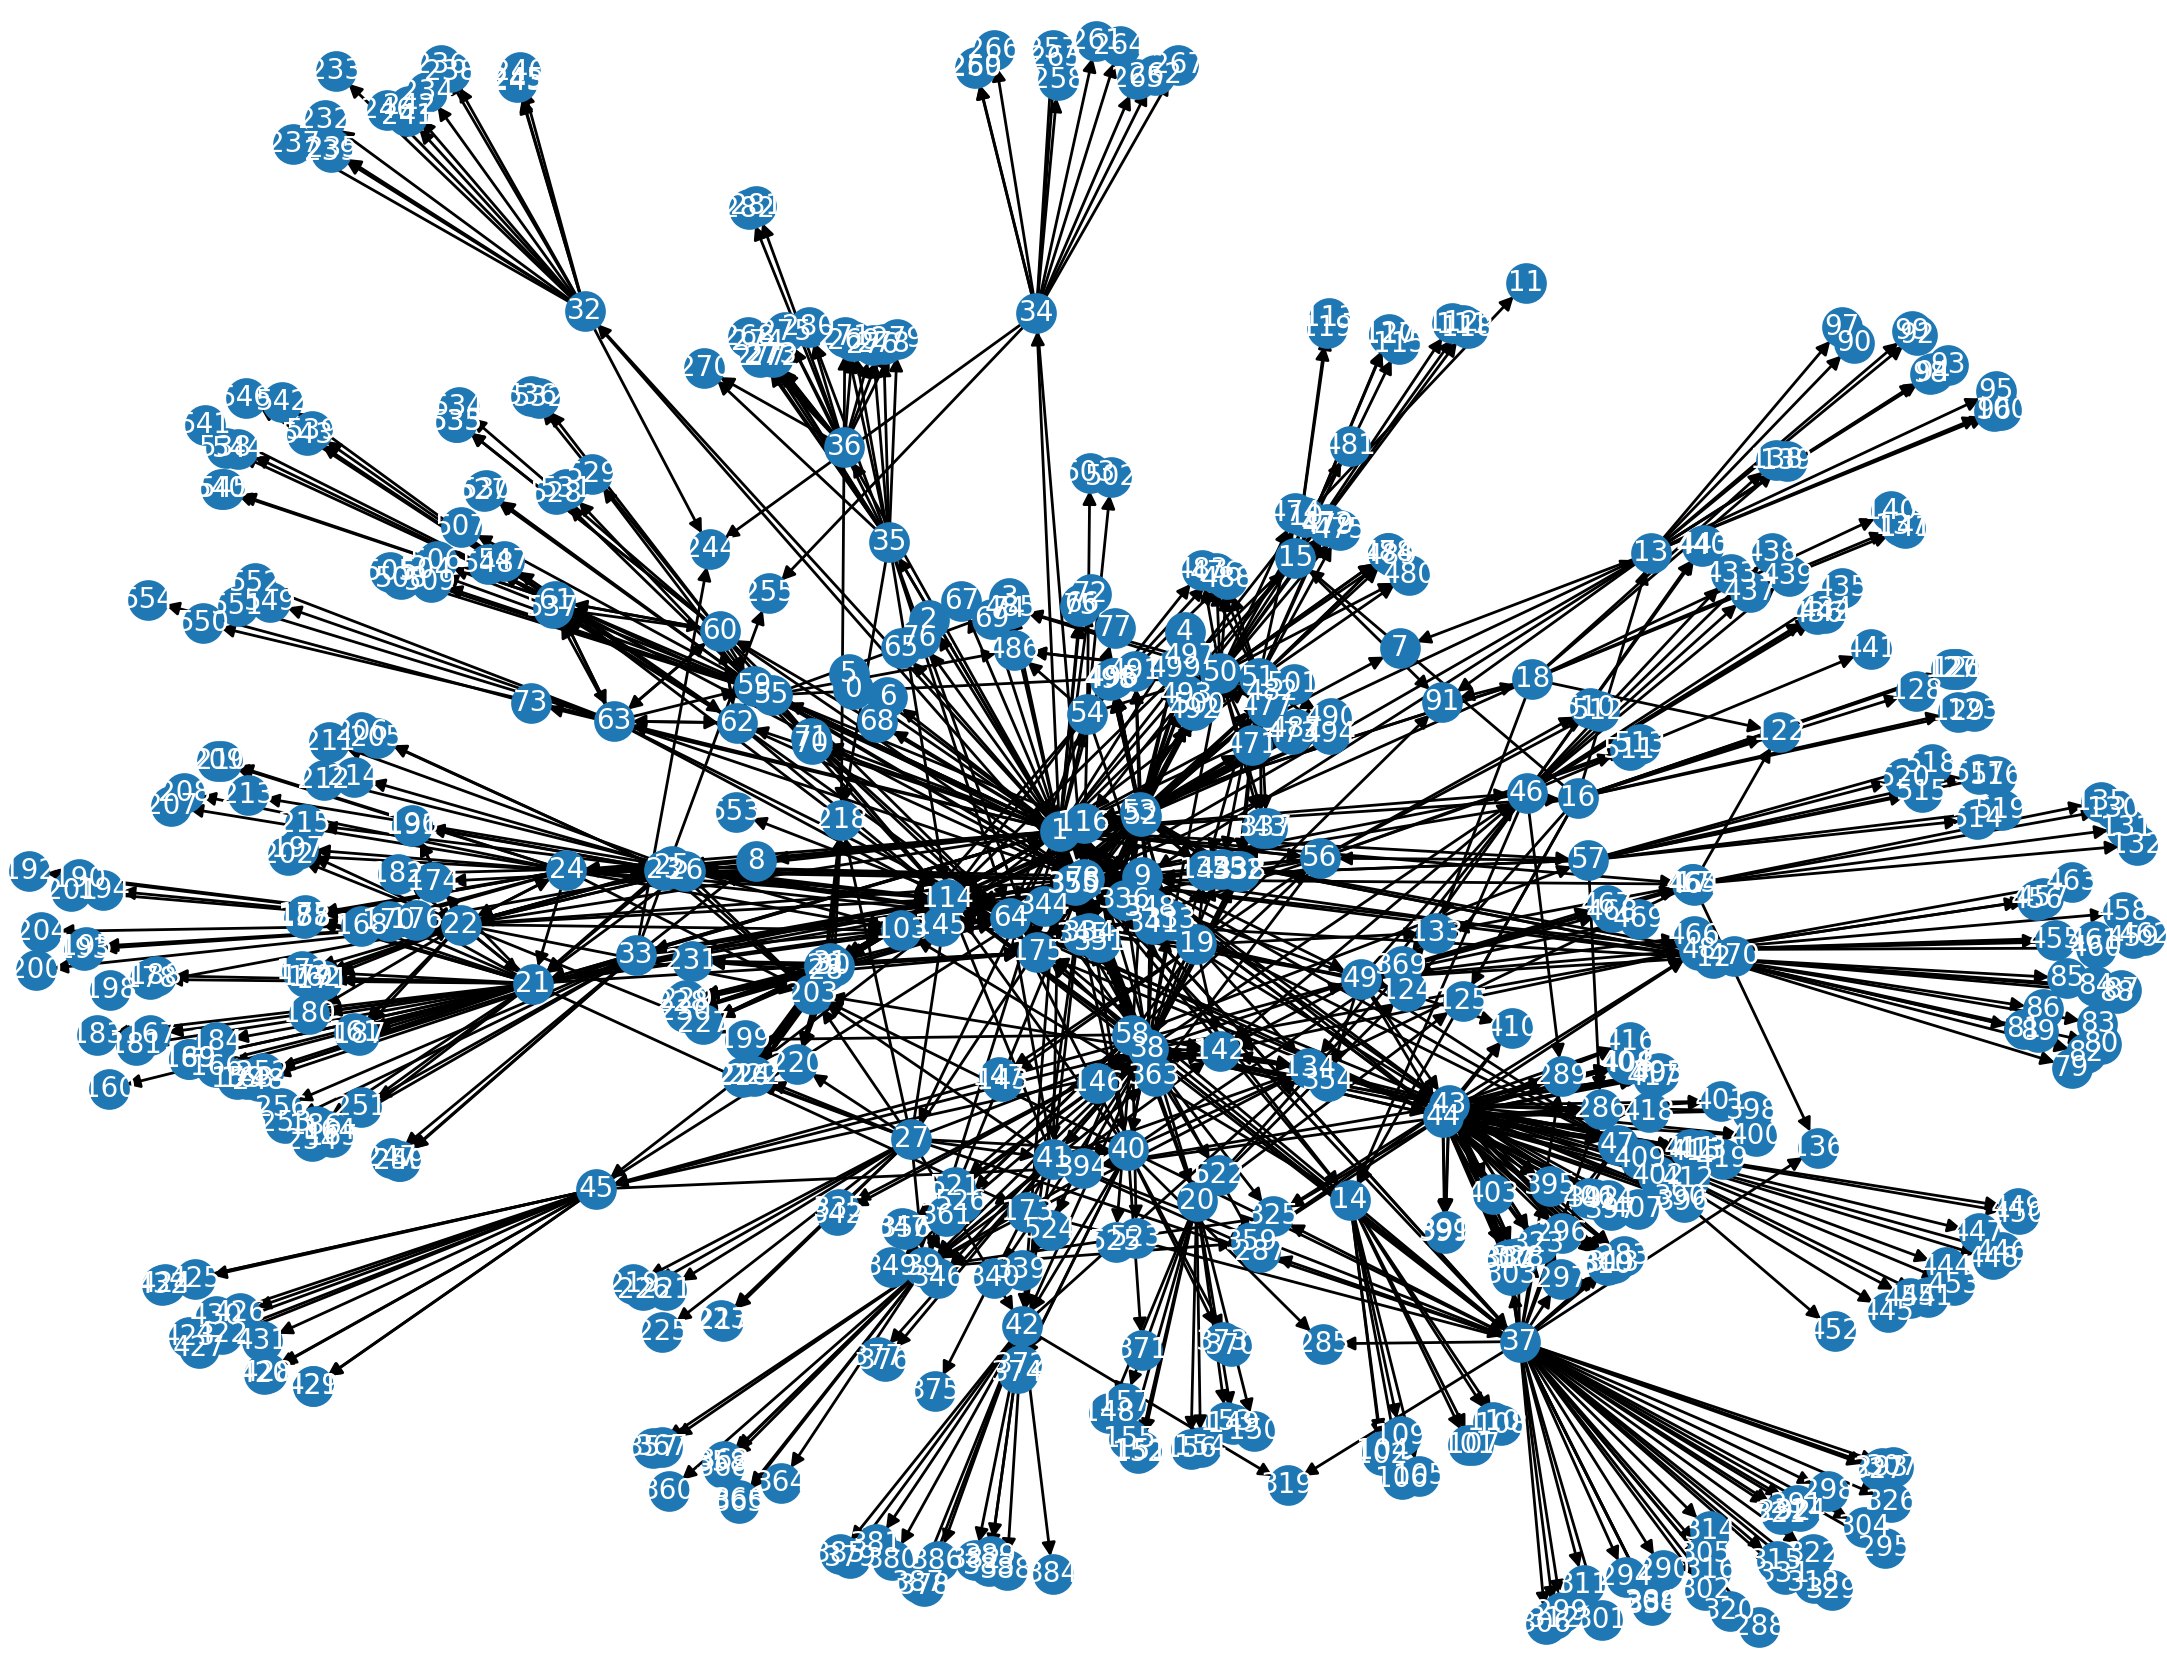
\includegraphics[width=0.7\textwidth]{img/yelp_n_final.png}}
\end{figure}
\end{frame}



\begin{frame}[fragile]\frametitle{Ukážka vygenerovaného testu}


\begin{itemize}
\item Test vygenerovaný pre LibreOffice StartCenter
\end{itemize}


\begin{center}
\begin{lstlisting}[language=Gherkin]
Scenario: libreoffice-startcenter: Spreadsheet
* Start: "libreoffice-startcenter" via command 
* Action: "click" "File" "menu"
* Action: "click" "New" "menu"
* State: "menu item" "Spreadsheet" "showing" is "True"
* OCR: "Spreadsheet" is shown on the screen
* Action: "click" "Spreadsheet" "menu item"
* State: "frame" "Untitled 1 - LibreOffice Calc" is shown
* OCR: "Untitled 1 - LibreOffice Calc" is shown 
\end{lstlisting}
\end{center}
\end{frame}

\begin{frame}[fragile]\frametitle{Výsledky práce}
 
 \begin{itemize}
 \item Proces generovania testov zahŕňa aj testovanie aplikácie
    \begin{itemize}
    \item \emph{upozornenie na určitý druh chyby v aplikácii už počas testovania}
    \item \emph{kroky na zreprodukovanie chyby}
    \end{itemize}
\vspace{2mm}
\item Otestovaných bolo 5 GUI aplikácií:
\begin{itemize}
    \item \emph{GNOME Help, GNOME Terminal}
    \item \emph{Gedit -- textový editor}
    \item \emph{Evince -- aplikácia na zobrazovanie dokumentov (\textit{.pdf, .xps})}
    \item \emph{LibreOffice StartCenter}
\end{itemize}
\vspace{2mm}
\item Preukázala sa schopnosť nástroja detekovať určité chyby:
\begin{itemize}
    \item \emph{pády aplikácie -- LibreOffice StartCenter}
    \item \emph{chyby plynúce z chybových hlásení aplikácie -- Evince, \\ Firefox (chyba nájdená pri testovaní GNOME Help)}
\end{itemize}
\vspace{2mm}
\item Zistené chyby v assistenčných technológiách (limity riešenia):
\begin{itemize}
    \item \emph{chyby prejavujúce sa pri rekurzívnom prehľadávaní aplikácie}
    \item \emph{zlé zaradenie prvkov v podstrome}
\end{itemize}
\vspace{2mm}
\item Nasadenie vygenerovaných testov v CI prostredí (\textit{RedHat})

\end{itemize}

\end{frame}

\bluepage{
Ďakujem za pozornosť
}

\appendix
\begin{frame}[fragile]\frametitle{Otázka oponenta}

\begin{block}{\vspace{2mm}\textbf{Is there a plan for further development of the test generation tool?}\vspace{2mm}}

\begin{itemize}
\item Spätná väzba z prezentácie práce vo firme Red Hat:
\begin{itemize}
\item \emph{automatizované testovanie aplikácií}
\item \emph{rýchle vygenerovanie základnej sady testov, ktorú je možné okamžíte nasadiť v prostredí CI}
\item \emph{integrácia OCR}
\end{itemize}
\item Možnosť testovania len určitého podstromu aplikácie
\item Možnosť pridania sady testovacích súborov

\end{itemize}

\end{block}
    
\end{frame}
\end{document}
